% ─────────────────────────────────────────────────────────────────────────────
%  Figure 1: τ-Sweep Divergence  (HEAS WSC 2026)
%  Two-panel standalone figure compiled to PDF.
%  Left  (a): Rank Reversal Rate (%) — line chart
%  Right (b): Cohen's h effect size — bar chart
% ─────────────────────────────────────────────────────────────────────────────
\documentclass[border=4pt]{standalone}

\usepackage{pgfplots}
\pgfplotsset{compat=1.18}
\usepackage{tikz}
\usetikzlibrary{positioning, shapes.geometric, arrows.meta}
\usepackage{xcolor}
\usepackage{mathptmx}   % Times New Roman for body text
\usepackage[T1]{fontenc}

% ── Palette ───────────────────────────────────────────────────────────────────
\definecolor{cEntropy}{HTML}{4D4D4D}   % dark grey  — semantic
\definecolor{cStep}   {HTML}{D6604D}   % orange-red — syntactic
\definecolor{cMean}   {HTML}{4DAF4A}   % green      — near-uniform
\definecolor{cHEAS}   {HTML}{2166AC}   % blue       — HEAS contract
\definecolor{cGrid}   {HTML}{E8E8E8}
\definecolor{cRef}    {HTML}{999999}

% ── Shared axis style ─────────────────────────────────────────────────────────
\pgfplotsset{
  fig1base/.style={
    width  = 6.8cm,
    height = 5.4cm,
    grid   = major,
    grid style     = {color=cGrid, line width=0.4pt},
    axis line style= {gray!60, line width=0.7pt},
    tick style     = {gray!60, line width=0.5pt},
    tick pos       = left,
    xlabel style   = {font=\small},
    ylabel style   = {font=\small},
    tick label style = {font=\footnotesize},
    title style    = {font=\small, at={(0,1.06)}, anchor=south west, xshift=0pt},
    legend style   = {
      font       = \scriptsize,
      draw       = gray!40,
      fill       = white,
      fill opacity= 0.92,
      text opacity= 1,
      inner sep  = 3pt,
      row sep    = 1pt,
    },
  }
}

\begin{document}
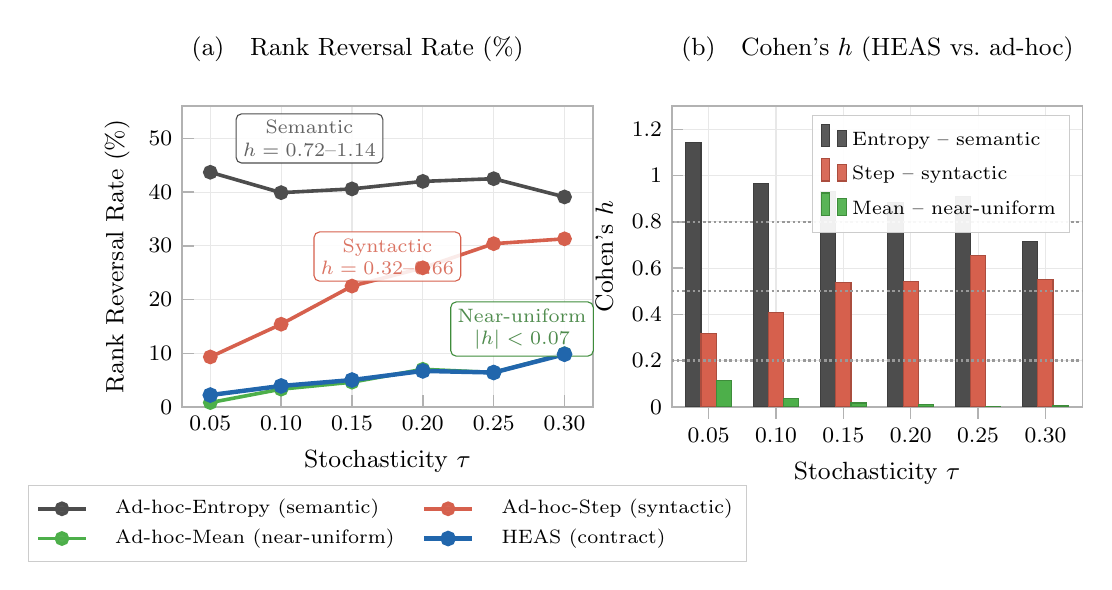
\begin{tikzpicture}

% ═════════════════════════════════════════════════════════════════════════════
% LEFT PANEL (a) — Rank Reversal Rate (%)
% ═════════════════════════════════════════════════════════════════════════════
\begin{axis}[
  fig1base,
  name   = panelA,
  title  = {(a)\quad Rank Reversal Rate (\%)},
  xlabel = {Stochasticity $\tau$},
  ylabel = {Rank Reversal Rate (\%)},
  xmin   = 0.03,  xmax = 0.32,
  ymin   = 0,     ymax = 56,
  clip   = false,
  xtick        = {0.05, 0.10, 0.15, 0.20, 0.25, 0.30},
  xticklabels  = {0.05, 0.10, 0.15, 0.20, 0.25, 0.30},
  scaled ticks = false,
  ytick  = {0, 10, 20, 30, 40, 50},
  legend style = {
    at             = {(0.5, -0.26)},
    anchor         = north,
    font           = \scriptsize,
    draw           = gray!40,
    fill           = white,
    fill opacity   = 0.95,
    text opacity   = 1,
    inner sep      = 3pt,
    row sep        = 0pt,
    column sep     = 8pt,
  },
  legend columns   = 2,
  legend cell align = left,
]

% Ad-hoc-Entropy (semantic)
\addplot[
  color      = cEntropy,
  mark        = *,
  mark size   = 2.0pt,
  line width  = 1.3pt,
] coordinates {
  (0.05, 43.7)(0.10, 39.9)(0.15, 40.6)(0.20, 42.0)(0.25, 42.5)(0.30, 39.1)
};
\addlegendentry{Ad-hoc-Entropy (semantic)}

% Ad-hoc-Step (syntactic)
\addplot[
  color      = cStep,
  mark        = *,
  mark size   = 2.0pt,
  line width  = 1.3pt,
] coordinates {
  (0.05,  9.3)(0.10, 15.4)(0.15, 22.5)(0.20, 25.9)(0.25, 30.4)(0.30, 31.3)
};
\addlegendentry{Ad-hoc-Step (syntactic)}

% Ad-hoc-Mean (near-uniform)
\addplot[
  color      = cMean,
  mark        = *,
  mark size   = 2.0pt,
  line width  = 1.3pt,
] coordinates {
  (0.05,  0.8)(0.10,  3.3)(0.15,  4.6)(0.20,  7.0)(0.25,  6.4)(0.30,  9.9)
};
\addlegendentry{Ad-hoc-Mean (near-uniform)}

% HEAS (contract)
\addplot[
  color      = cHEAS,
  mark        = *,
  mark size   = 2.0pt,
  line width  = 1.6pt,
] coordinates {
  (0.05,  2.2)(0.10,  3.9)(0.15,  5.0)(0.20,  6.7)(0.25,  6.4)(0.30,  9.8)
};
\addlegendentry{HEAS (contract)}

% ── Regime annotation boxes ──────────────────────────────────────────────────
\node[
  draw = cEntropy, rounded corners = 2pt,
  fill = white, fill opacity = 0.88,
  inner sep = 2.5pt, font = \scriptsize, align = center,
  text = cEntropy,
] at (axis cs: 0.12, 50) {Semantic\\$h=0.72$--$1.14$};

\node[
  draw = cStep, rounded corners = 2pt,
  fill = white, fill opacity = 0.88,
  inner sep = 2.5pt, font = \scriptsize, align = center,
  text = cStep,
] at (axis cs: 0.175, 28) {Syntactic\\$h=0.32$--$0.66$};

\node[
  draw = cMean!80!black, rounded corners = 2pt,
  fill = white, fill opacity = 0.88,
  inner sep = 2.5pt, font = \scriptsize, align = center,
  text = cMean!70!black,
] at (axis cs: 0.270, 14.5) {Near-uniform\\$|h|<0.07$};

\end{axis}


% ═════════════════════════════════════════════════════════════════════════════
% RIGHT PANEL (b) — Cohen's h  (HEAS vs. ad-hoc)
% ═════════════════════════════════════════════════════════════════════════════
\begin{axis}[
  fig1base,
  name       = panelB,
  at         = (panelA.east),
  anchor     = west,
  xshift     = 1.0cm,
  title      = {(b)\quad Cohen's $h$ (HEAS vs.\ ad-hoc)},
  xlabel     = {Stochasticity $\tau$},
  ylabel     = {Cohen's $h$},
  xmin       = -0.55,  xmax = 5.55,
  ymin       = 0,      ymax = 1.30,
  xtick      = {0, 1, 2, 3, 4, 5},
  xticklabels= {0.05, 0.10, 0.15, 0.20, 0.25, 0.30},
  ytick      = {0, 0.2, 0.4, 0.6, 0.8, 1.0, 1.2},
  ybar,
  bar width  = 5.5pt,
  legend pos = north east,
  legend cell align = left,
]

% Entropy bars
\addplot[
  fill = cEntropy, draw = cEntropy!80!black,
  bar shift = -5.5pt,
] coordinates {
  (0, 1.144)(1, 0.967)(2, 0.932)(3, 0.885)(4, 0.909)(5, 0.715)
};
\addlegendentry{Entropy -- semantic}

% Step bars
\addplot[
  fill = cStep, draw = cStep!80!black,
  bar shift = 0pt,
] coordinates {
  (0, 0.318)(1, 0.407)(2, 0.538)(3, 0.544)(4, 0.656)(5, 0.552)
};
\addlegendentry{Step -- syntactic}

% Mean bars
\addplot[
  fill = cMean, draw = cMean!80!black,
  bar shift = 5.5pt,
] coordinates {
  (0, 0.116)(1, 0.036)(2, 0.017)(3, 0.010)(4, 0.002)(5, 0.006)
};
\addlegendentry{Mean -- near-uniform}

% ── Cohen's h reference lines ────────────────────────────────────────────────
\draw[cRef, densely dotted, line width=0.9pt]
  (axis cs:-0.55, 0.2) -- (axis cs:5.55, 0.2)
  node[right, font=\scriptsize, color=cRef, xshift=-1pt] {\,small};

\draw[cRef, densely dotted, line width=0.9pt]
  (axis cs:-0.55, 0.5) -- (axis cs:5.55, 0.5)
  node[right, font=\scriptsize, color=cRef, xshift=-1pt] {\,medium};

\draw[cRef, densely dotted, line width=0.9pt]
  (axis cs:-0.55, 0.8) -- (axis cs:5.55, 0.8)
  node[right, font=\scriptsize, color=cRef, xshift=-1pt] {\,large};

\end{axis}

\end{tikzpicture}
\end{document}
